\section{Configuração no ESP 32}

Para a realização da atividade prática, usamos um ESP32 de 30 pinos, uma protoboard de 400 pontos, um LED RGB, três resistores de 390 ohms, quatro cabos macho-fêmea e um cabo micro-USB.

Na protoboard, dispomos o LED RGB em uma região bem próxima à linha negativa que fica na beirada da placa. Para que possamos conectar o cátodo o LED nessa linha. Os outros pinos são colocados arbitrariamente em colunas diferentes.

Na coluna de cada pino RGB, conectamos os resistores 390 ohms para evitar que o LED queime. Os terminais de cada resistores podem se manter na mesma coluna, mas não devem ser conectados na coluna do terminais de outros resistores.

\begin{figure}[H]
    \centering
    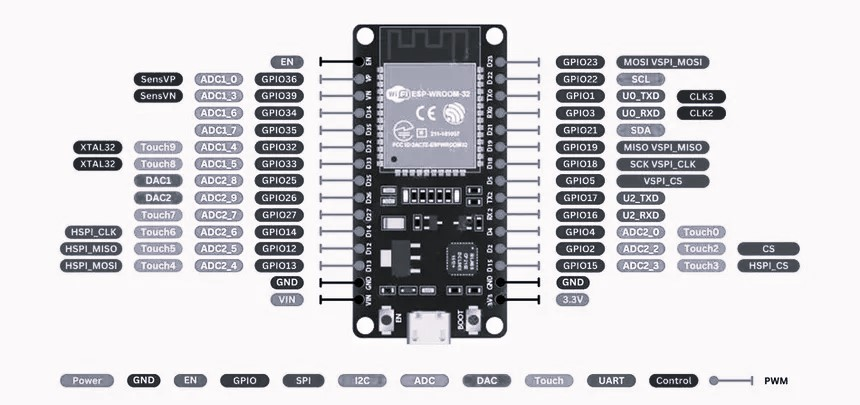
\includegraphics[width=0.5\linewidth]{img/esp32_pinout.png}
    \caption{Pinout do ESP32.}
    \label{fig:esp32-pinout}
\end{figure}

Escolhemos os pinos 18, 20 e 21 para conectar aos terminais do LED para as cores vermelho, verde e azul, respectivamente. Então, conectamos esses pinos na coluna do terminal dos resistores que estão conectados ao terminal de cada cor na protoboard utilizando os cabos macho-fêmea. Por fim, conectamos o cátodo do LED RGB no GND do ESP32.

\begin{figure}[H]
    \centering
    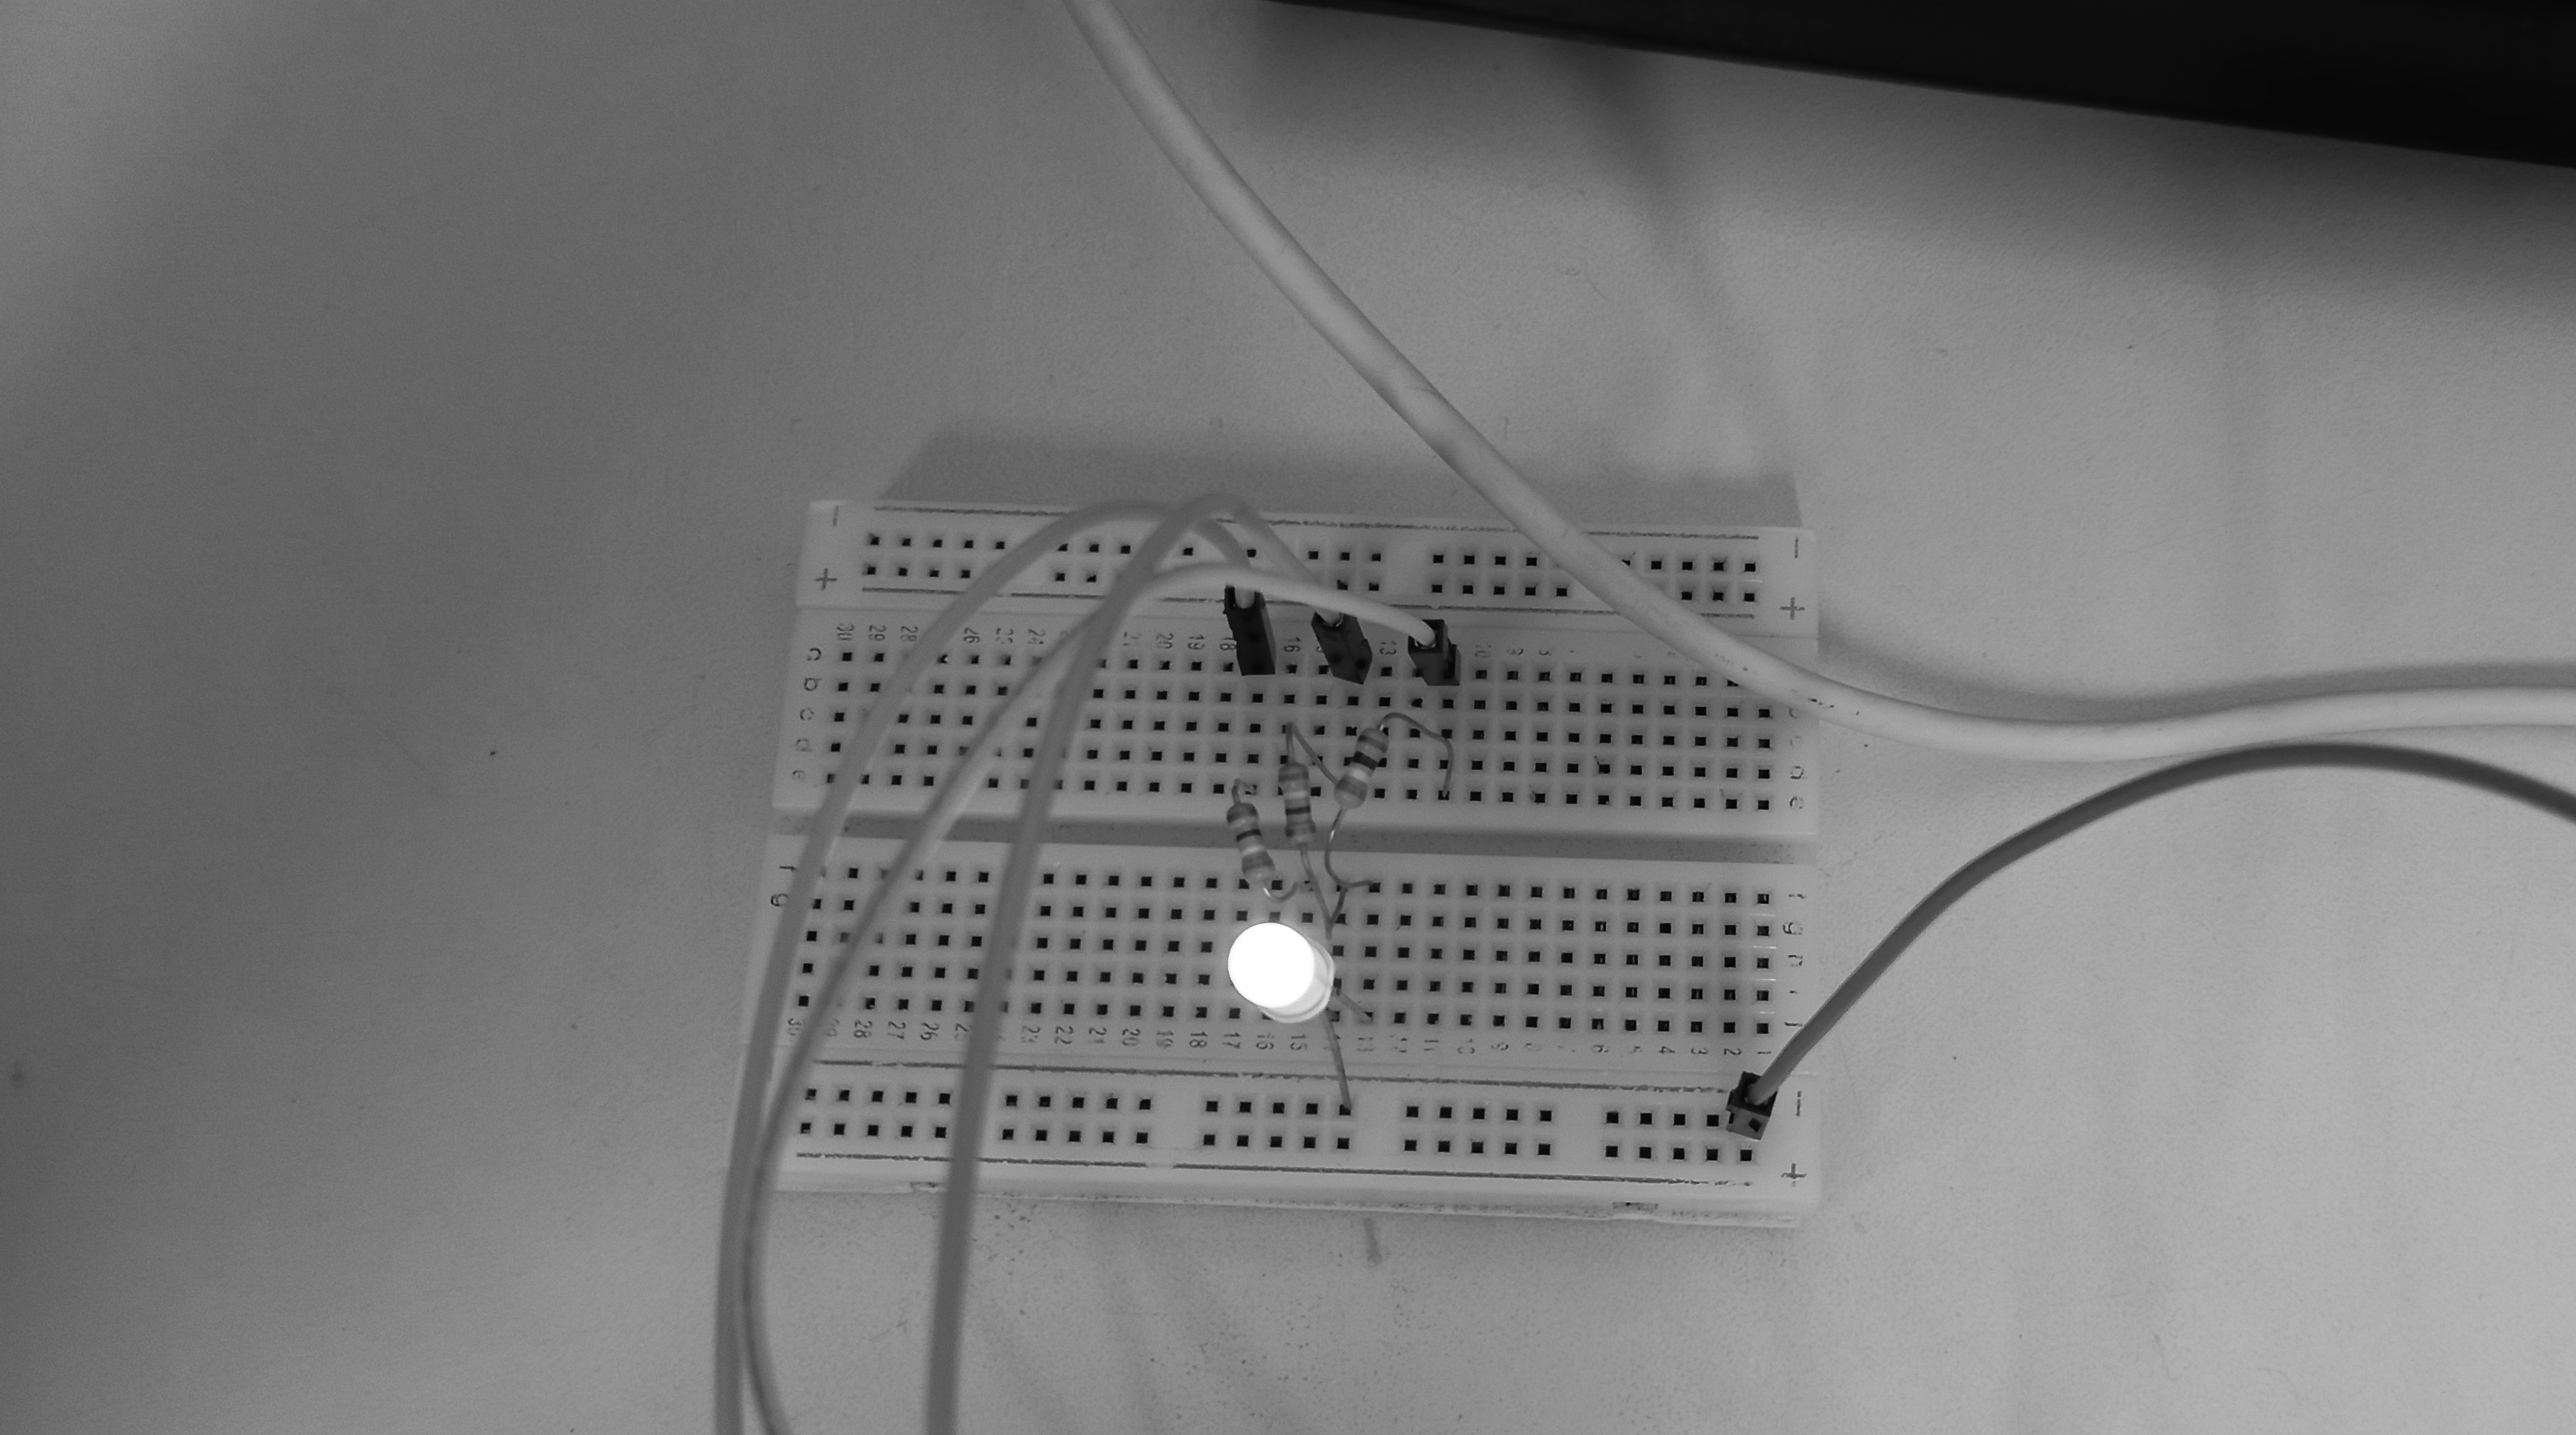
\includegraphics[width=0.5\linewidth]{img/protoboard_config.jpg}
    \caption{Configuração na protoboard.}
    \label{fig:protoboard-config}
\end{figure}